%!TEX root = chi14grammatical.tex
\begin{figure*}[th]
	\begin{subfigure} {1.3\columnwidth}
			\centering
	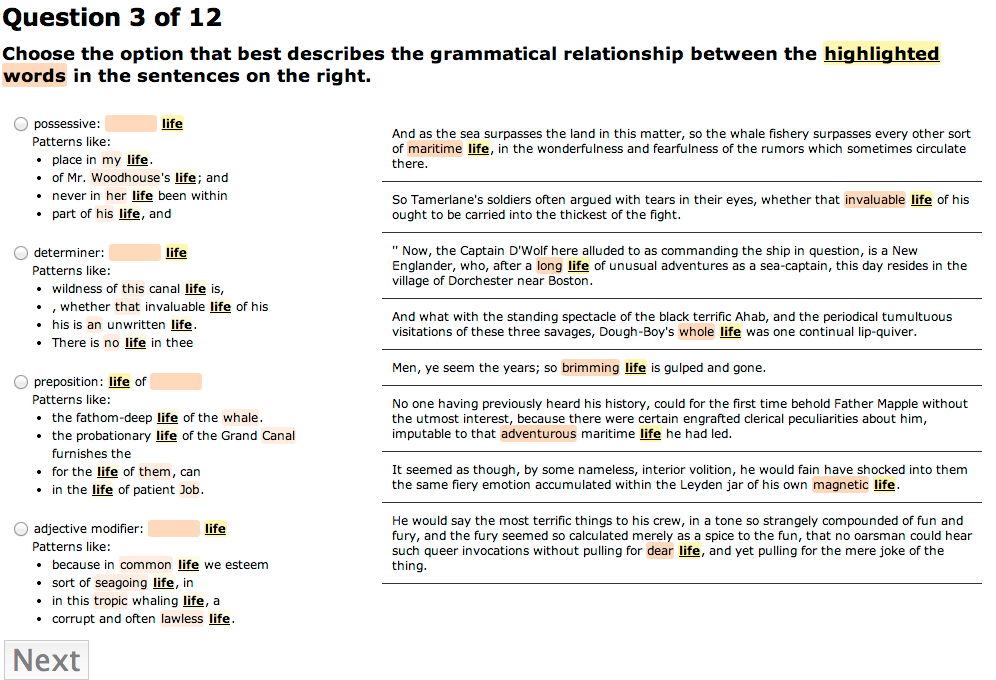
\includegraphics[width=1.2\columnwidth]{fig/task}
	\caption{\label{fig:task} An example of an identification task in the \emph{phrases} condition for the relationship \code{amod(life, \_\_\_)} (where different adjectives modify the noun `life'). The correct answer is `adjective modifier' (4th option), and the remaining 3 options are distractors.}
	\end{subfigure}
	\qquad\qquad\qquad
	\begin{subfigure}{0.7\columnwidth}
		\begin{subfigure}{0.7\columnwidth}
				\centering
		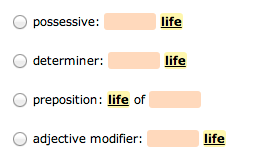
\includegraphics[width=0.9\columnwidth]{fig/baseline-choices}
	    \caption {The same options as they appear in the \emph{baseline} condition. \label{fig:baseline-choices}}
	    \end{subfigure}


	    \begin{subfigure}{0.7\columnwidth}
	    	\centering
	    	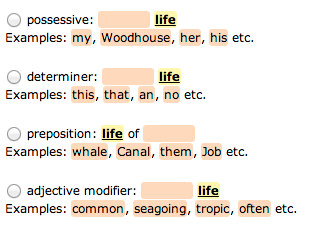
\includegraphics[width=0.9\columnwidth]{fig/words-choices}
	        \caption {The same options as they appear in the \emph{words} condition. \label{fig:words-choices}}
	    \end{subfigure}
	\end{subfigure}
\caption{\label{fig:choices} The appearance of the choices shown in the three experiment conditions.}
\end{figure*}

% \section{Related Work}

% Trees are the traditional representation of syntactic parses, so trees are often the focus of query input for collections of syntactically parsed data.

% Several approaches have adopted XML representations and the associated query language families of XPATH and SPARQL. For example, LPath augments XPath with additional tree operators to give it further expressiveness \cite{lai2010querying}.

